\section{When to Use @ngrx/store}
When to use @ngrx/store can be a very opiniated item to consider. State as we
know it, is a single data object, that can be accessed anywhere within the app.
How this happens, changes from one state management framework to another, but
the core is the same. However, the difficulty, is that state, being that it
exists outside of the component, can contain quite a bit of bloat.

\mybox{It is interesting to note, that the original implementation of Flux
was created by Facebook back in 2014\footnote{This video contains https://www.youtube.com/watch?v=nYkdrAPrdcw this fact}.
It was because they had a bug with regards to the chat counter, that just kept
on coming back. It would mention that a user did not read a message, but that
wasn't true. Flux was the architecture they came up with in order to solve this
bug. It's important to understand the history of where Flux came from, when
trying to understand how to move forward using it. It's important to also
realize, that the issue, wasn't they weren't able to solve it, it is that the
bug kept coming back. Flux solved it, due to it's straight forward way of
solving multiple components interacting with each other.

``It is important to remember, that a store is about creating an in-memory client
side database, which is a user-specific slice of the database, and use that
data to derivce View Models from it on the client.''
}

\subsection{Redux as evolution on Flux}
Redux solved the same problem Flux did. However, it simplified the process.
Without going into too much detail and instead showing a photo, Redux simplified
the problem it solved, and made it easier to implement:

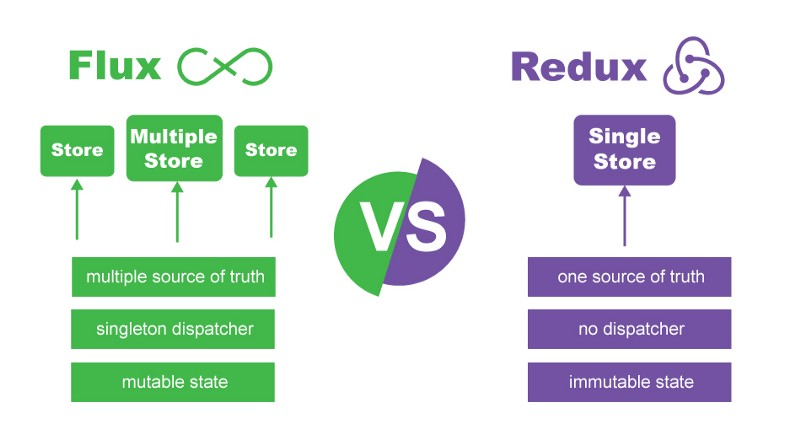
\includegraphics[width=12.1cm, height=9cm]{./state/when-to-use-ngrx/flux_v_redux}

\subsection{ An Example of an @ngrx/store }

For instance, let's say that we have a user-settings data-access feature. Our
folder file structure might look like the following:

\begin{forest}
  [libs
    [px-illustrator
      [data-access
        [user-settings
          [src
            [lib
              [\_+state
                [\_user-settings.actions.ts,file]
                [\_user-settings.effects.spec.ts,file]
                [\_user-settings.effects.ts,file]
                [\_user-settings.facade.mock.ts,file]
                [\_user-settings.facade.spec.ts,file]
                [\_user-settings.facade.ts,file]
                [\_user-settings.reducer.spec.ts,file]
                [\_user-settings.reducer.ts,file]
                [\_user-settings.selectors.ts,file]
              ]
              [\_px-illustrator-data-access-user-settings.module.ts,file]
              [\_px-illustrator-data-access-user-settings.module.spec.ts,file]
              [\_px-illustrator-data-access-user-settings-testing.module.spec.ts,file]
            ]
            [\_index.ts,file]
            [\_test.ts,file]
          ]
          [\_karma.conf,file]
          [\_README.md,file]
          [\_tsconfig.lib,file]
          [\_tsconfig.lib.json,file]
          [\_tsconfig.spec.json,file]
          [\_tslint.json,file]
        ]
      ]
    ]
  ]
\end{forest}


This, of course, would be in an enterprise setting, which honestly this book
is geared towards. However, it definitely strikes home a very good point. There
is a ton of bloat to creating a store. Even once a developer get's over the hill
of creating state, and get's used to it, it's still a lot to manage, and one
just has to ask, does it always make sense?

\subsection{ Addressing the Problems State Alleviates }
First and foremost, I think it would be most effective if we were to directly
jump into the problems that state solves:
\begin{enumerate}
  \item Avoiding Multiple Actors
  \item Avoid Extraneous @Inputs
  \begin{enumerate}
    \item Pass down multiple levels to child, and send change back to parent
    \item Siblings in a tree, might have to pass up and over
  \end{enumerate}
  \item Stops Event Bussing /marginpar{Look more into this one}
  \item Decouples component interaction. Component does not know what changed,
  only knows what changed it.
  \item Allows for Component interaction via the Observable Pattern
  \item Client Side Cache if needed.
  \item Place to Put Temporary UI State
\end{enumerate}

These would be in my humble opinion, the 7 things that state has to offer. If a
component were to be able to interact with another component on that page, by
altering it's data, it should have state.

\subsection{ Attachments Service - Story Time }
There are some very unique cases, where perhaps state shouldn't be used. I for
one always felt that state has a bit of bloat. However, after discussing with
team members, I have begun to see the way they think. This particular situation
was about a feature for attachments that the app needed. In particular,
multiple components on the same page, would have attachments. If a service or
@ngrx/store was not used, there would be alot of repitition across the app. This
led to the dillema, should a service, or @ngrx/store be used.

\subsection{ Business Requirments }
One, is that multiple components on the same page were to use this attachments
service. Second, is that we want to show the user when a certain attachment is
loading, and when it is no longer loading.

\subsection{ Argument for using a Service }
In truth, the attachments were meant to be self contained within a singular
component. This would have made the service as very simple. However, based on
the business requirements, we would have to create a double nested correlation
id. This means that a double nested correlation id pattern had to be created.
One, to make sure that different components do not affect each other. Two, the
id produced on the front end, is different than the id produced on the backend.
We need to create an id that can be used by both. This is done by creating a
second Uuid, that is nested within the first one. I.e. \ a dictionary inside of a
dictionary.

So, really in this situation, there is arguably nothing that the store has to
offer. However, what has happened, is that using @ngrx/store, we are now
comfortable with the API for @ngrx/entity. In addition, we have a single place
where we expect all of our data to be. Creating a service like this, might make
sense for the person spending the time thinking through the problem. However,
for any other person, it will be an incredibly uncomfortable experience reading
through your code. @ngrx/store therefore at this point takes on it's new life
as a way to make sure code is consistent, even if it isn't the right choice for
your app.

\subsection{ What Comes Out From Our Back and Forth }
Truly, any situation, wherein a data request is made from the back end, it
should go into our store.
